\documentclass[12pt,a4paper]{article}
\usepackage[utf8]{inputenc}
\usepackage[ngerman]{babel}
\usepackage[T1]{fontenc}
\usepackage{amsmath}
\usepackage{amsfonts}
\usepackage{amssymb}
\usepackage{graphicx}
\usepackage{subfigure}
\author{Alexander Binsmaier, Manuel Mende, Yaroslav Direy}
\title{Auswertung MPGA -- günstige und ungünstige Parametrisierungen}

\begin{document}
\maketitle
\tableofcontents
\section{Allgemeines Vorgehen}
Um die Parametrisierung der Algorithmen gegeneinander auszuwerten, muss eine Vergleichsbasis geschaffen werden. Eine Möglichkeit ist es, den genetischen Multi-Populations-Algorithmus ohne Migration laufen zu lassen. Basierend auf den Ergebnissen dieses Durchlaufs können dann unterschiedliche Konfigurationen des Algorithmus ausgeführt und verglichen werden. Um die Komplexität zu relativieren, wurden einige Einschränkungen getroffen. Die Algorithmen sollen immer auf acht Chromosome umfassende Populationen angewendet werden. Die Parametrisierung des zugrunde liegenden genetischen Algorithmus ist identisch -- abgesehen von den verwendeten Fitnessfunktionen -- und die durchlaufenden Generationen werden auch konstant gehalten. Eine geeignete Anzahl Generationen wird durch die migrationslose Ausführung festgelegt. Als Variationsparameter verbleiben die Anzahl an Migrationen und die Anzahl an Generationen bis zur nächsten Migration. Zudem kann die Strategie variiert werden.
Primär existiert die uneingeschränkte Migration (unrestricted), bei der jede Population in jede andere Population migrieren kann. Als zweite Möglichkeit besteht die Ring-Migration. Hier wird semantisch nicht zusammenhängend in die nächste Population migriert. Die auf Nachbarschaft basierende Migrationsstrategie erlaubt eine Migration nur, wenn Ziel- und Quellpopulation auf der selben Seite -- also vor oder hinter -- der Parklücke liegen. 
Die Auswertung erfolgt im Anschluss und betrachtet vor allem die Entwicklung der mittleren Populationsfitness über die Epochen. Speziell gilt das Interesse, wie schnell ein akzeptables Fitness-Niveau erreicht wird. Auch die Testfälle der Ergebnispopulation werden entsprechend in die Bewertung mit eingehen, sowie deren Ähnlichkeit innerhalb der Populationen.

\section{Migrationsfreier Durchlauf}
Primär dient die migrationsfreie Ausführung des Algorithmus der Festlegung einer Vergleichsbasis. Zudem kann die Geschwindigkeit der Konvergenz des Algorithmus als Indiz für die Anzahl notwendiger Generationen für die migrierenden Ausführungen verwendet werden. Die Ausführung erfolgt dabei mit den selben Realisierungen der genetischen Algorithmen -- identische Fitnessfunktionen in den einzelnen Populationen, gleiche Parametrisierung der Rekombination und Mutation -- wie in den Durchläufen mit Migration. Um ein Generationslimit festzulegen, wir eine sehr hohe Anzahl Generationen gewählt. Für jede Population werden 5000 Epochen durchlaufen.
\begin{figure}
\centering
	\subfigure[Mittlere Fitness\label{fig:plain_fit}]{
		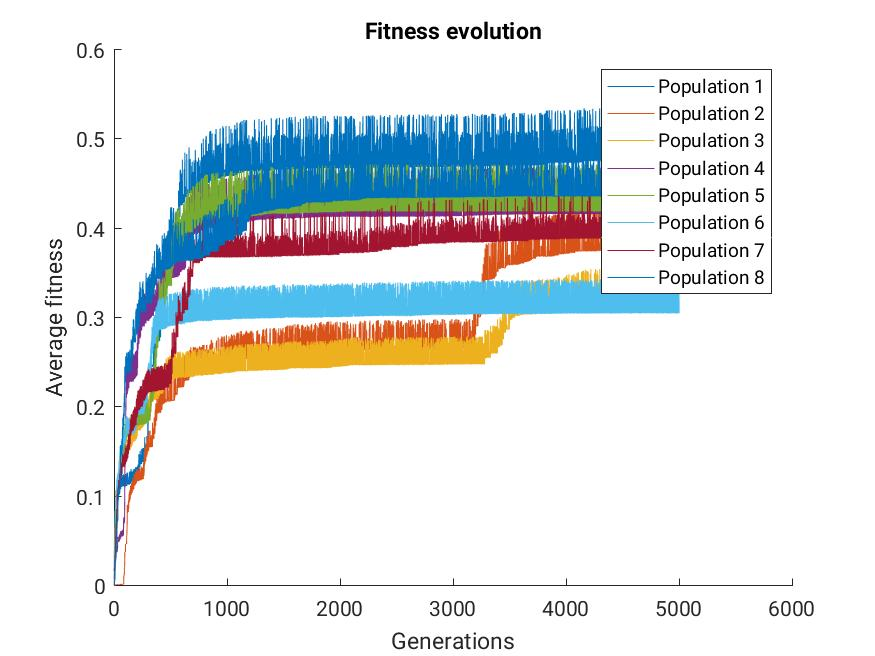
\includegraphics[width=.45\textwidth]{plain-fit.jpg}
	}
	\subfigure[Ergebnispopulation\label{fig:plain_tcs}]{
		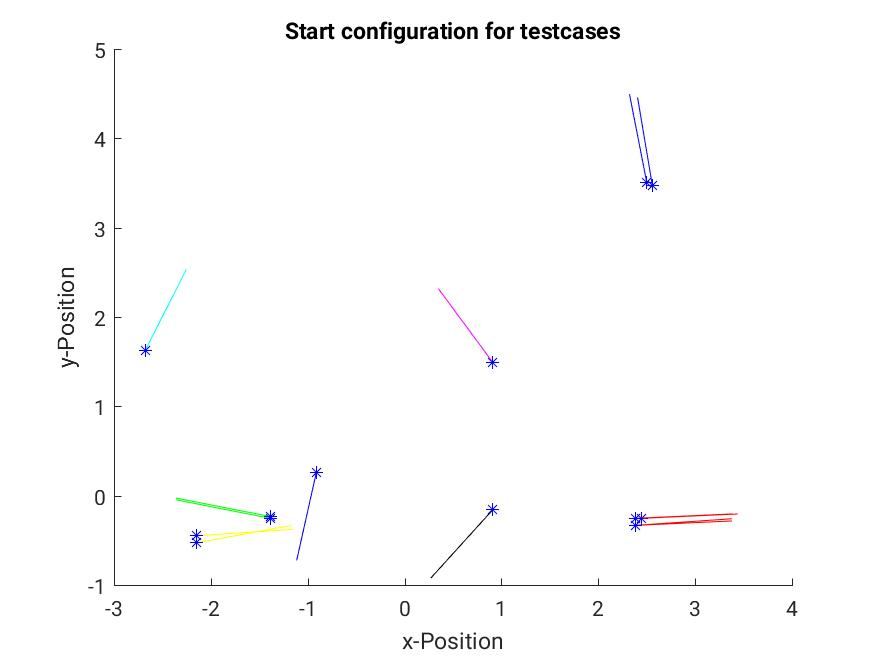
\includegraphics[width=.45\textwidth]{plain-tcs.jpg}
	}
	\caption{Migrationsfreie Evolution mit 5000 Generationen}
\end{figure}

\subsection{Entwicklung der Fitness}
Wie in Abbildung \ref{fig:plain_fit} ersichtlich, konvergiert die gemittelte Fitness der Populationen zu einem maximalen Wert von etwa $0.5$, welcher für die beste Population bereits ab 1000 Generationen erreicht wird. Daher wurde als Generationslimit für die migrierenden Ausführungen 1000 Generationen gewählt. Zwar treten in einigen Generationen auch später noch Verbesserungen auf. Jedoch besteht die Hoffnung, dass ein migrierender Ansatz hier schneller zu besseren Werten führt.

\subsection{Testfälle}
Natürlich ist es erforderlich, dass die Fitness schnell konvergiert. Dennoch muss auch beachtet werden, dass die resultierenden Testfälle auch die Anforderungen erfüllen. Die Populationen wurden nach diversen Gesichtspunkten ausgewählt. So kann das Fahrzeug vor oder hinter der Parklücke liegen und tendenziell nach oben, unten, links oder rechts orientiert sein. Aus der Kombination von Lage und Orientierung ergeben sich acht Populationen, die jeweils charakteristische Chromosome hervorbringen. Diese müssen in der Ergebnispopulation auftreten.
Abbildung \ref{fig:plain_tcs} zeigt eine Ergebnispopulation ohne Migration. Deutlich sind die entsprechenden Klassen erkennbar.

\section{Vergleiche}
\subsection{Migrationsraten}
Allgemein hat es sich als schlecht erwiesen, einen großen Teil der Population zu tauschen. Bei jedem Migrations-Schritt wird die Gesamtfitness in ihrer Entwicklung zurück geworfen. Bei großen Zyklen wird dies besonders deutlich, bei kleineren Zyklen entsteht ein Rauschen ohne ersichtlichen Fitnessgewinn. Werden sieben von acht Chromosome pro Population migriert ist keine Verbesserung erkennbar, wie Abbildung \ref{fig:high_migrate} verdeutlicht. 
Ein Austausch von 50\% der Population führt schon zu einer Steigerung der Gesamtfitness. Mit einem Migrationsabstand von 50 Generationen sieht man aber immer noch einen eklantanten Einbruch der Fitness (siehe Abbildung \ref{fig:mid_migrate}).\\
Im Vergleich zu anderen Parametrisierungen ist diese allerdings gering und im Besonderen schlechter als migrationsfreie Evolution. In Ausnahmefällen kann es dennoch zu einer sprunghaften Steigerung führen, allerdings tritt dieses Phänomen nur selten und rein zufällig auf.
\begin{figure}
\centering
	\subfigure[Hohe Migrationsrate\label{fig:high_migrate}]{
		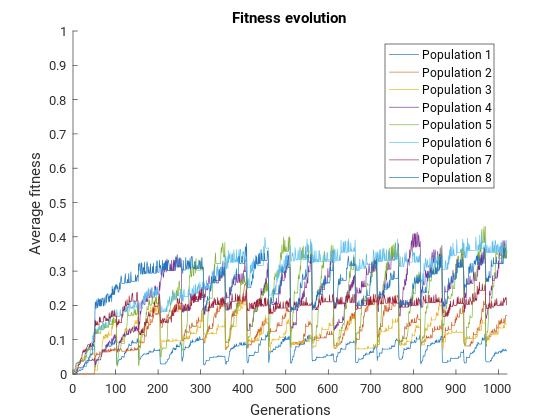
\includegraphics[width=.45\textwidth]{high_migrate.jpg}
	 }
	 \subfigure[Mittlere Migrationsrate\label{fig:mid_migrate}]{
		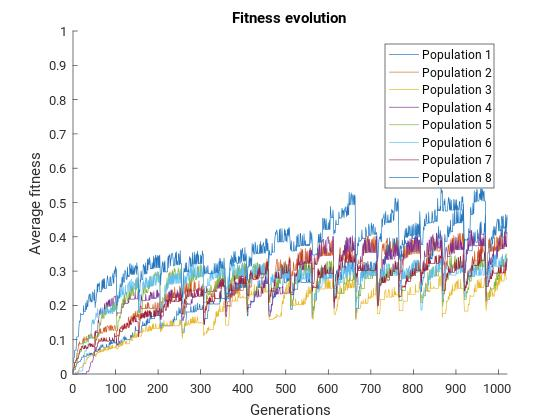
\includegraphics[width=.45\textwidth]{mid_migrate.jpg}
	 }
	 \caption{Migration alle 50 Generationen}
\end{figure}

\subsection{Migrationszyklen}
% Generell ist eine migRate von 1 gut. Häufige Migration sorgt für schnelle Konvergenz (cs=1). Seltene Migration (cs=100) sorgt für homogene Ergebnispopulationen, die Konvergenz ist nicht ganz so schnell. Dennoch ist die Geschwindigkeit in Relation zum plain-Ansatz besser.
Eine gering gewählte Anzahl Migrationsvorgänge in jedem Migrationszyklus führt zu stärkerer Fitness-Konvergenz.\\
Abbildung \ref{fig:small_cycles} zeigt kleine Migrationszyklen der Größe 1. Es wird also nach jedem Evolutionsschritt migriert. Man erkennt eine sich schnell verbessernde Gesamtfitness. Bei 250 Generationen vor der nächsten Migration in Abbildung \ref{fig:big_cycles} ist auch ein Aufwärtstrend erkennbar, allerdings nur wenig schneller als bei der isolierten Evolution aus Abbildung \ref{fig:plain_fit}.
\begin{figure}
\centering
\subfigure[Kleine Migrationszyklen\label{fig:small_cycles}]{
	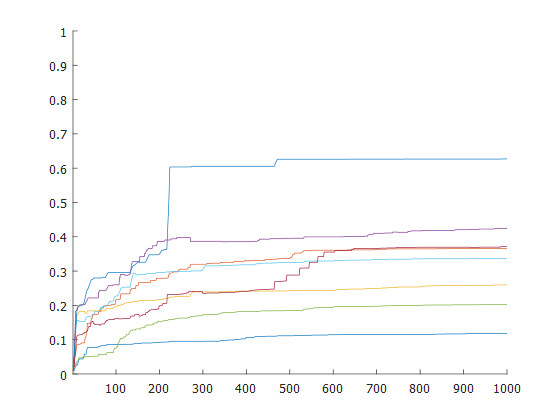
\includegraphics[width=.45\textwidth]{policy-ring_migRate-1_cycleSize-1-fit_alt.jpg}
}
\subfigure[Große Migrationszyklen\label{fig:big_cycles}]{
	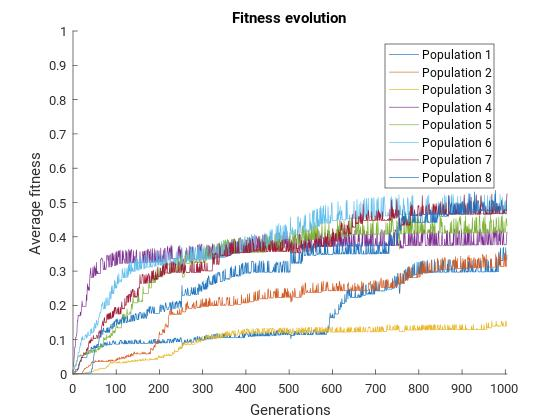
\includegraphics[width=.45\textwidth]{policy-ring_migRate-1_cycleSize-250-fit.jpg}
}
\caption{Fitness unterschiedlicher Migrationszyklus-Längen}
\end{figure}

\subsection{Qualität Der Ergebnisse}
Vergleicht man hingegen die Ergebnispopulationen, erkennt man eine stärkere Anpassung der generierten Testfälle and die erwünschte Testfall-Klasse bei größeren Migrationszyklen. Dies ist zu erwarten, da der genetische Algorithmus bei kleinen Migrationszyklen nicht die Chance bekommt, neu migrierte Individuen in seine Population aufzunehmen beziehungsweise aus ihr auszugrenzen. Die hellblaue Population in \ref{fig:big_cycles_tcs} schwankt stark, selbiges gilt für die rote und die magenta-farbige Population. Bei den Testfällen in Abbildung \ref{fig:small_cycles_tcs} hingegen weist lediglich die gelbe Population stark unterschiedliche Individuen auf.\\
Betrachtet man die resultierenden Testfälle von Abbildung \ref{fig:big_cycles_tcs} genauer, passen sie gut in das spezifizierte Testfall-Schema. Jede Population lässt sich einer Testfallklasse zuordnen.

\begin{figure}
\centering
\subfigure[Kleine Migrationszyklen\label{fig:small_cycles_tcs}]{
	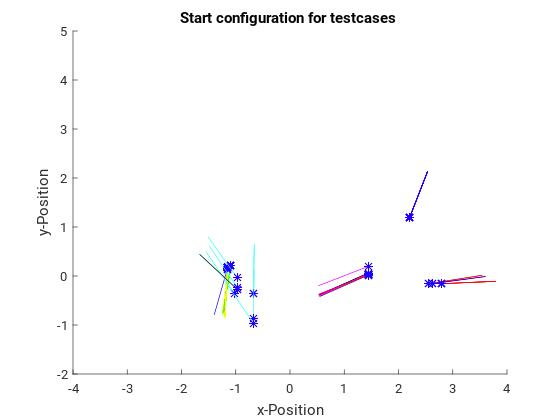
\includegraphics[width=.45\textwidth]{policy-ring_migRate-1_cycleSize-1-tcs.jpg}
}
\subfigure[Große Migrationszyklen\label{fig:big_cycles_tcs}]{
	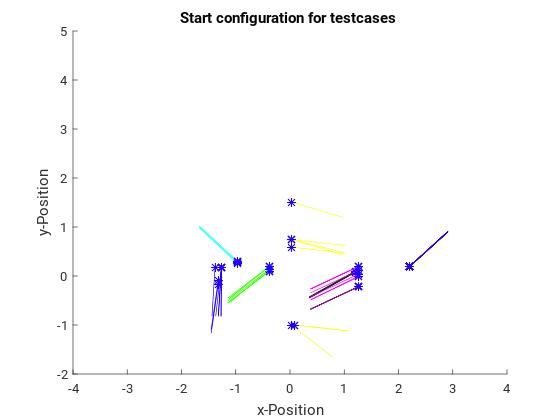
\includegraphics[width=.45\textwidth]{policy-ring_migRate-1_cycleSize-250-tcs.jpg}
}
\caption{Ergebnispopulation verschiedener Migrationszyklus-Längen}
\end{figure}

\subsection{Migration Policies}
Um Migration Policies vergleichen zu können, muss man sich zuerst auf eine Festlegung der übrigen Konfigurationsparameter einigen. Hier nehmen wir aufgrund der zuvor erörterten Ergebnisse folgende Parametrisierung: Alle 100 Epochen wird 1 Chromosom pro Population migriert. Die bietet gute Konvergenzgeschwindigkeit und hinreichend gute Einhaltung der Testfall-Klassen.\\
Zuerst werden die beiden semantisch zusammenhangslosen Policies miteinander Verglichen. Weder die Unrestricted noch die Ring Policy berücksichtigen bei der Migrations-Partner-Wahl, ob es einen semantischen Zusammenhang zwischen den Beiden Partnern gibt. Unrestricted wählt eine beliebige Population als Partner und Ring wählt stets die der Implementierung nach als nächste dem MPGA hinzugefügte aus. Zu erwarten ist demnach ein Einbruch der durchschnittlichen Fitness einer Population, wenn ein komplett ungeeignetes Chromosom aus einer semantisch vollkommen fremden Population in jene migriert.\\
Abgebildet ist dieser Vergleich in Abbildung \ref{fig:cmp_policy:chaos}. Man sieht, dass der größte Unterschied darin liegt, bei welcher Variante die erste Population einen relativ stabilen Fitnesswert annimmt. Dagegen erreicht bei beiden Varianten die letzt Population ihren stabilen Fitnesswert bei ungefähr 600 - 700 Epochen.\\
Danach vergleichen wir die Unrestricted Policy mit der Neighbour Policy, die einzige, die in der Lage ist, semantische Zusammenhänge bei der Wahl des Migrationsziel zu berücksichtigen. Dies rührt daher, dass in unserem Fall Nachbarschaft als Klassenzugehörigkeit definiert ist. Die Klassen sind hier eingeteilt in Testfälle, welche versuchen das Fahrzeug auf der linken Seite des Parkplatzes starten zu lassen, und andere, die dasselbe auf der rechten Seite zu erzielen versuchen.\\
Das Ergebnis dieses Vergleichs sieht man in Abbildung \ref{fig:cmp_policy:semantic}. Man sieht sofort, dass die Neighbour Policy deutlich besser abschneidet als die Unrestricted Policy. Die durchschnittlichen Fitnesswerte erreichen im Allgemeinen schneller ihren stabilen Endwert. Aufgrund obiger Ausführung entspricht dies vollkommen den Erwartungen.

\begin{figure}
\centering
\subfigure[Unrestricted Policy]{
	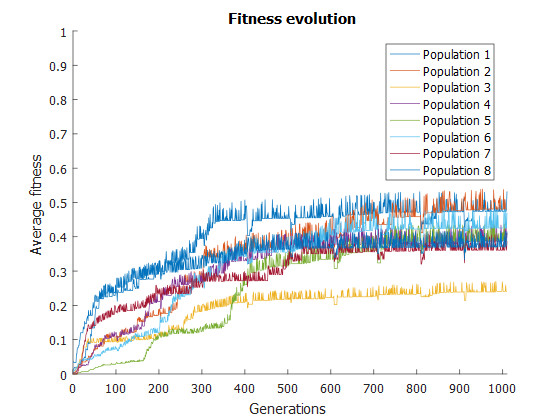
\includegraphics[width=.45\textwidth]{mig_unres_cs100_mr1.jpg}
	\label{fig:cmp_policy:unres1}
}
\subfigure[Ring Policy]{
	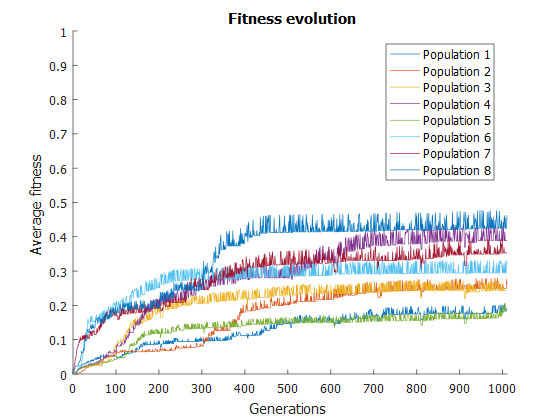
\includegraphics[width=.45\textwidth]{mig_ring_cs100_mr1.jpg}
	\label{fig:cmp_policy:ring}
}
\caption{Vergleich: Semantisch Zusammenhanglose Policies}
\label{fig:cmp_policy:chaos}
\end{figure}

\begin{figure}
\centering
\subfigure[Unrestricted Policy]{
	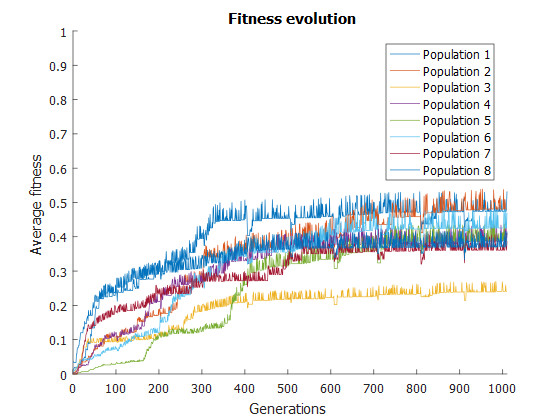
\includegraphics[width=.45\textwidth]{mig_unres_cs100_mr1.jpg}
	\label{fig:cmp_policy:unres2}
}
\subfigure[Neighbour Policy]{
	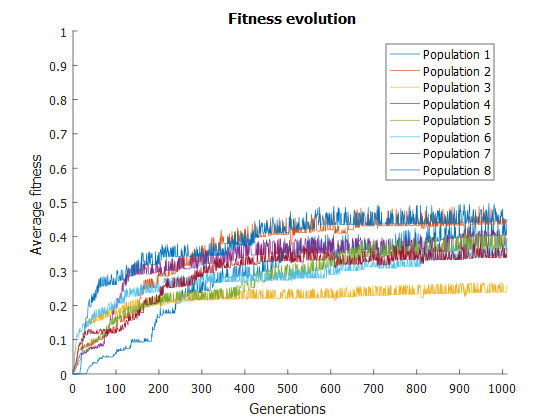
\includegraphics[width=.45\textwidth]{mig_neigh_cs100_mr1.jpg}
	\label{fig:cmp_policy:neigh}
}
\caption{Vergleich: Unrestricted vs Neighbour Policy}
\label{fig:cmp_policy:semantic}
\end{figure}

\subsection{MPGA vs GA}
Zuletzt ist der normale Genetic Algorithm dem Multi-Population Genetic Algorithm gegenüberzustellen.\\
Hier sieht man in Abbildung \ref{fig:cmp_spga_mpga_fit}, dass mit einer sinnvollen Wahl von Konfigurationsparametern der Multi-Population Genetic Algorithm die Erwartungen erfüllt und schneller konvergiert als die normale GA Implementierung. Die Parametrisierung ist hier 1 Chromosom alle 100 Epochen mittels Neighbour Migration zu migrieren.\\
Beim Vergleich der generierten Testfälle, lässt sich beobachten, dass die vom MPGA generierten sich populationsübergreifend wesentlich ähnlicher sind, als die, der 8 normalen GA Durchläufe. Dies ist in Abbildung \ref{fig:cmp_spga_mpga_tcs} dargestellt. Nichts desto trotz erfüllen sie beide hinreichend gut die Testfall-Klassen. Der Unterschied kommt lediglich daher, dass durch die Migration die in Abbildung \ref{fig:cmp_spga_mpga_tcs:mpga} gezeigten Chromosome mit höherer Wahrscheinlichkeit ähnliche y-Koordinaten haben. Diese fließen lediglich durch das Ergebnis der Simulation in die Fitness eines Chromosoms mit ein - im Gegensatz zur x-Koordinate, die bewusst nach 'rechts' oder 'links' vom Parkplatz mittels entsprechender Fitnessfunktion gelenkt wird - und sind deswegen mit höherer Wahrscheinlichkeit durch die Migration bedingt ähnlich.
\begin{figure}
\label{fig:cmp_spga_mpga_fit}
\centering
\subfigure[Normaler GA\label{fig:cmp_spga_mpga_fit:spga}]{
	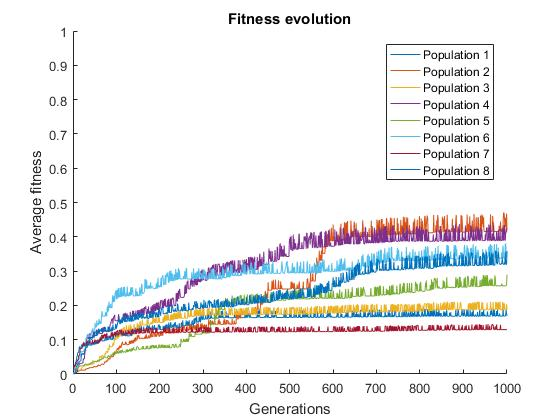
\includegraphics[width=.45\textwidth]{mig_free_fit.jpg}
}
\subfigure[MP GA\label{fig:cmp_spga_mpga_fit:mpga}]{
	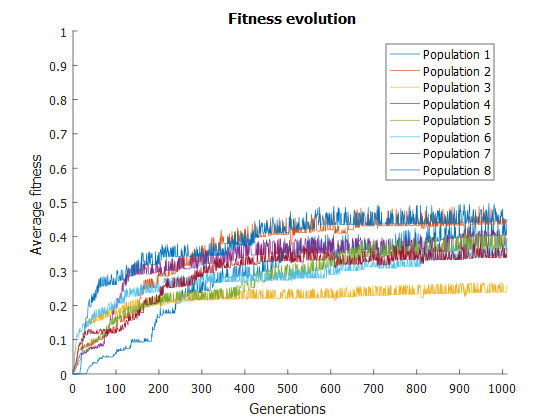
\includegraphics[width=.45\textwidth]{mig_neigh_cs100_mr1.jpg}
}
\caption{Vergleich: Konvergenz Normaler vs MP Genetic Algorithm}
\end{figure}

\begin{figure}
\label{fig:cmp_spga_mpga_tcs}
\centering
\subfigure[Normaler GA\label{fig:cmp_spga_mpga_tcs:spga}]{
	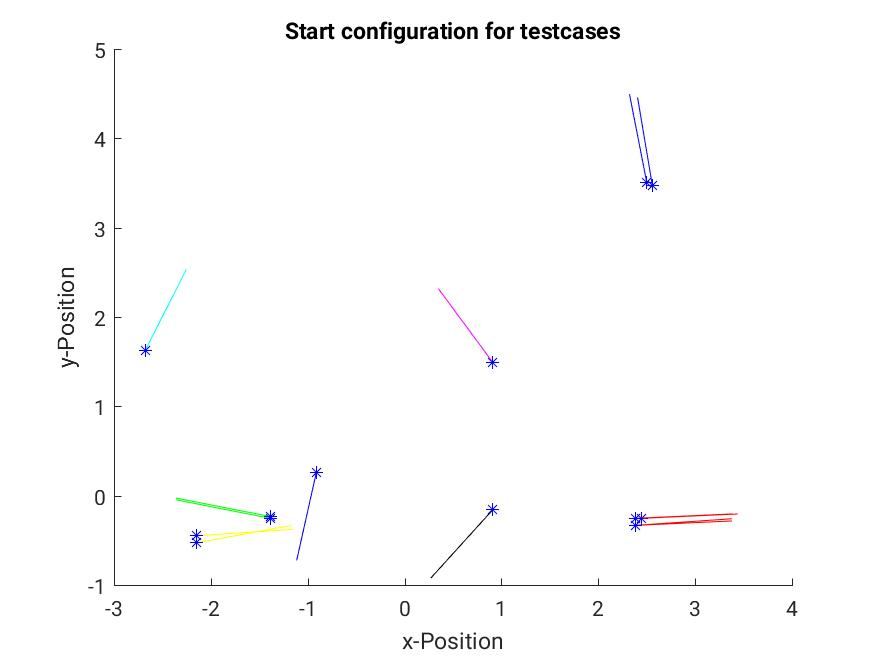
\includegraphics[width=.45\textwidth]{plain-tcs.jpg}
}
\subfigure[MP GA\label{fig:cmp_spga_mpga_tcs:mpga}]{
	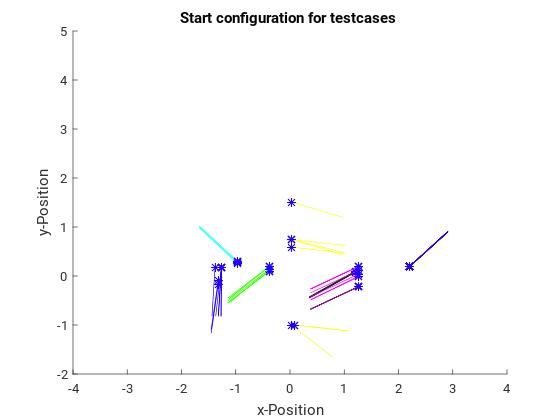
\includegraphics[width=.45\textwidth]{policy-ring_migRate-1_cycleSize-250-tcs.jpg}
}
\caption{Vergleich: Testfälle Normaler vs MP Genetic Algorithm}
\end{figure}

\section{Zusammenfassung}
Schlussfolgernd fällt nun sofort auf, dass das einzige unumstritten klar herausgearbeitete Ergebnis die Tatsache ist, dass kleine Migrationsraten vorzuziehen sind.\\
Des Weiteren lässt sich ebenso davon ausgehen, dass die Neighbour Policy den anderen Policies vorzuziehen ist, auch wenn hier der Unterschied verhältnismäßig klein ausfällt.\\
Beim Migrationszyklus gilt es, die Laufzeit gegen die Ähnlichkeit der Ergebnisse zu den erwünschten Testfall-Klassen abzuwägen. Hier macht eine Größenordnung von 50 Epochen zwischen zwei Migrationen insofern am meisten Sinn, dass das schnelle Konvergenzverhalten von minimalen Migrationszyklen noch ersichtlich ist und dennoch die generierten Testfälle klar ihren Klassen zuzuordnen sind.
\end{document}
